\documentclass[pressentation,10pt,aspectratio=169,xcolor=table, colorlinks=true]{beamer}
\usepackage[utf8]{inputenc}
\usepackage[T1]{fontenc}
\usepackage{graphicx}
\usepackage{longtable}
\usepackage{wrapfig}
\usepackage{rotating}
\usepackage[normalem]{ulem}
\usepackage{amsmath}
\usepackage{amssymb}
\usepackage{capt-of}
\usepackage{overlock}\usepackage[english]{babel}
\usepackage{tikz, pgfplots}\usepackage{smartdiagram}
\usetikzlibrary{arrows,shapes,positioning,mindmap,decorations.pathreplacing,backgrounds,overlay-beamer-styles,calc,3d,fit,matrix,graphs, arrows.meta}
\usepgfplotslibrary{groupplots}
\pgfplotsset{/pgf/number format/assume math mode=true}\usepackage{csquotes}
\usepackage[outline]{contour} % glow around text
\contourlength{1.4pt}
\usepackage{listofitems}
\usepackage[citestyle=verbose, backend=biber]{biblatex}\addbibresource{refs.bib}
\usepackage[type={CC}, modifier={by-sa}, version={4.0},]{doclicense}
\pgfplotsset{compat=1.17}
\usepackage{minted}\usemintedstyle{emacs}\usepackage[]{tcolorbox}
\newtcolorbox[auto counter]{work}[1][]{colback=black!5!white,colframe=black!50!white,fonttitle=\sffamily\bfseries,title=Work}

\hypersetup{
  colorlinks = true
}

\AtBeginSection{%
  % \begin{frame}<beamer>[plain]
  %   \frametitle{Outline}
  %   \tableofcontents[sectionstyle=show/shaded,subsectionstyle=show/shaded]
  % \end{frame}
  \begin{frame}<beamer>[plain]
    \frametitle{Outline}
    \begin{columns}[onlytextwidth,T]
        \begin{column}{.45\textwidth}
            \tableofcontents[sectionstyle=show/shaded,subsectionstyle=show/shaded, sections=1-4]
        \end{column}
        \begin{column}{.45\textwidth}
            \tableofcontents[sectionstyle=show/shaded,subsectionstyle=show/shaded, sections=5-6]
        \end{column}
    \end{columns}
\end{frame}
  \addtocounter{framenumber}{-1}
}%

\AtBeginSubsection{%
  % \begin{frame}<beamer>[plain]
  %   \frametitle{Outline}
  %   \tableofcontents[sectionstyle=show/shaded,subsectionstyle=show/shaded]
  % \end{frame}
  \begin{frame}<beamer>[plain]
    \frametitle{Outline}
    \begin{columns}[onlytextwidth,T]
        \begin{column}{.45\textwidth}
            \tableofcontents[sectionstyle=show/shaded,subsectionstyle=show/shaded, sections=1-4]
        \end{column}
        \begin{column}{.45\textwidth}
            \tableofcontents[sectionstyle=show/shaded,subsectionstyle=show/shaded, sections=5-6]
        \end{column}
    \end{columns}
\end{frame}
  \addtocounter{framenumber}{-1}
}%

\usetheme{default}
\usecolortheme[snowy]{owl}
\setbeamertemplate{navigation symbols}{}{}
\setbeamertemplate{footline}[frame number]
\setbeamertemplate{itemize item}{$\bullet$}
\setbeamertemplate{itemize subitem}{$\star$}
\setbeamercolor{block body}{parent=normal text,use=block title,bg=black!5,}
\setbeamercolor{block title}{fg=black, bg=gray}
\setbeamertemplate{blocks}[rounded][shadow=false,] 

\DeclareMathOperator{\softmax}{softmax}
\DeclareMathOperator{\reshape}{reshape}

\author[M. Fauvel]{Mathieu FAUVEL}
\date{\today}
\title{UE Apprentissage SIA S9}
\subtitle{Supervise Learning}
\institute{CESBIO, Universit{\'e} de Toulouse, CNES/CNRS/INRAe/IRD/UPS, Toulouse, FRANCE}
\begin{document}
\maketitle

\begin{frame}
  \frametitle{Outline}
    \begin{columns}[onlytextwidth,T]
        \begin{column}{.45\textwidth}
            \tableofcontents[hideallsubsections, subsectionstyle=shaded, sections=1-4]
        \end{column}
        \begin{column}{.45\textwidth}
            \tableofcontents[hideallsubsections, subsectionstyle=shaded, sections=5-6]
        \end{column}
    \end{columns}
\end{frame}

\section{Introduction}

\begin{frame}
  \frametitle{Myself}
  \begin{itemize}
  \item Contact: mathieu.fauvel@inrae.fr
    
  \item CV:
    \begin{itemize}
    \item [2004-2007] Ph.D. degree in Signal and Image Processing from the INP, Grenoble \& the University of Iceland
    \item [2007-2008] Assistant Professor Grenoble
    \item [2008-2010] Post-doc position at INRIA - MISTIS Team
    \item [2010-2011] Assistant Professor Toulouse
    \item [2011-2018] Associate Professor at DYNAFOR \& INP, Toulouse
    \item [Since 2018] Research (CRCN) at CESBIO, INRAe
    \end{itemize}
  \item Research interests are:
    \begin{center}
      Machine learning for environmental/ecological monitoring
    \end{center}
  \end{itemize}
\end{frame}

\begin{frame}
  \frametitle{Course Objectives}
  \begin{itemize}
  \item Learn basics of modern machine learning
  \item Understand how each step works
    \begin{itemize}
    \item Data préparation
    \item Model definition
    \item Optimization step
    \end{itemize}
  \item Implement various Deep Learning models in PyTorch
  \item Application to Computer Vision
  \end{itemize}
\end{frame}

\begin{frame}
  \frametitle{What is Supervised (Machine) Learning ?}
  \begin{columns}[c]
    \begin{column}{0.5\linewidth}
      \begin{itemize}
      \item <1-> \textbf{Artificial Intelligence}
        \centerline{\em Perform human tasks using computers and algorithms}
      \item <2-> \cite{mitchelllearning}:
        \begin{center}
          \emph{Machine Learning is defined as the capacity of a computer program to improve its performance measure with observations}
        \end{center}
      \item <3-> \textbf{Deep Learning}
        \begin{itemize}
        \item Lot of data data
        \item Complex model
        \item High performance computing
        \end{itemize}
      \end{itemize}
    \end{column}

    \begin{column}{0.5\linewidth}
      \begin{center}
        \begin{tikzpicture}[scale=0.5]
          \draw[fill=yellow!40] (2.75,0) ellipse (6.4 and 3.2);
          \draw[fill=blue!40] (1,0) ellipse (4 and 2);
          \draw[fill=red!30] (-1,0) ellipse (1.6 and 0.8);
          
          \draw (4,2.25) node {\textbf{\small Artificial Intelligence}};
          \draw (1.7,1.05) node {\textbf{\small Machine Learning}};
          \draw (-1,0) node {\small \textbf{DL}};
        \end{tikzpicture}
      \end{center}
    \end{column}
  \end{columns}
\end{frame}


\begin{frame}
  \frametitle{Main Notations}
  \begin{block}{Data}
    \begin{itemize}
    \item Observed data \(\mathbf{x}\in \mathbb{R}^d\), called \emph{input variables} or \emph{predictors}.
    \item Data to be predicted \(y\in \mathbb{R}^p\), called \emph{output variables} or \emph{responses}.
    \end{itemize}
  \end{block}

  \begin{block}<2->{Learning Problem}
    \begin{itemize}
    \item If \(y\) are quantitative data: \emph{regression} and \(y\in\mathbb{R}^p\).
    \item If \(y\) are categorical data:  \emph{classification} and \(y\in\{C_1, \ldots, C_C\}\) with \(C_i\) refers to the \(i^{th}\) category.
    \end{itemize}
  \end{block}

  \begin{block}<3->{Prediction function}
    \begin{align*}
      f_{\boldsymbol{\theta}}: \mathbb{R}^d & \to  \mathbb{R}^p\\
      \mathbf{x} &  \mapsto  y
    \end{align*}
  \end{block}
\end{frame}

\begin{frame}
  \frametitle{Online References}

  \begin{itemize}
  \item \cite{zhang2021dive}
    
  \item \cite{prince2023understanding}

  \item \cite{mlbook2022}

  \item \cite{pml1Book}

  \item \cite{pml2Book}
  \end{itemize}
  
\end{frame}

\section{Introductory Example}
% Predict function
% Loss and Objective functions
% Gradient
% Optimization and Batch optim

\subsection{Linear model for regression}

\begin{frame}[fragile]
  \frametitle{Univariate linear model}
  \begin{columns}
    \begin{column}{0.5\linewidth}
      \begin{itemize}
      \item  \(f(x) = wx +b\)  and \(\boldsymbol{\theta} = (w,b)\)     
      \item Loss function: \(\ell \big(f(x_i),y_i\big) = \big(f(x_i) - y_i\big)^2\)
      \item Objective function: \[\mathcal{L} = \frac{1}{n} \sum_{i=1}^n \ell_i\]
      \item Gradients update: \(\boldsymbol{\theta}^{t+1} = \boldsymbol{\theta}^{t} - \eta\nabla_{\boldsymbol{\theta}}\mathcal{L}\)
        \begin{align*}
          \frac{\partial \mathcal{L}}{\partial w} & = & \frac{2}{n}\sum_{i=1}^n x_i(wx_i +b-y_i)\\
          \frac{\partial \mathcal{L}}{\partial b} & = & \frac{2}{n}\sum_{i=1}^n (wx_i +b-y_i)
        \end{align*}
      \end{itemize}
    \end{column}
    \begin{column}<2>{0.5\linewidth}
      \begin{work}
        Implement the 1D regression in pytorch of the following function:
        \[f(x)=2x-1\]

        Do the notebook:

        \begin{center}
          \textcolor{orange}{regression\_1d\_toy.ipynb}
        \end{center}
      \end{work}
    \end{column}
  \end{columns}
\end{frame}

\begin{frame}[fragile]
  \frametitle{Multivariate linear model}
  \begin{columns}
    \begin{column}{0.55\linewidth}
      \begin{itemize}
      \item \(f(\mathbf{x}) = \mathbf{w}^\top\mathbf{x} + b\) and \(\boldsymbol{\theta} = (\mathbf{w}, b)\)
        
      \item Same loss and objective function and so same gradient updates \ldots
      \item<2-> We can use other loss function

        \begin{center}
          \begin{tikzpicture}
            \begin{axis}[domain=-3:3, samples=200, grid, very thick, footnotesize, ymin=0, ymax=4.5, xmin=-3,xmax=3, legend pos=outer north east, legend cell align=left]
              \addplot[orange] {0.5*x*x};
              \addplot[blue] {abs(x)};
              \addplot[dashed, green] {abs(x) <= 1 ? 0.5*x^2 : (abs(x) - 0.5)};
              \addplot[purple] {1-exp(-x*x)};
              % \legend{$\ell(f(\mathbf{x}_i), y_i)= (f(\mathbf{x}_i), y_i)^2$, $\ell(f(\mathbf{x}_i)- y_i)= |f(\mathbf{x}_i)- y_i|$}
              \legend{\((f(\mathbf{x}_i)-y_i)^2\), \(|f(\mathbf{x}_i)-y_i|\), H(\(f(\mathbf{x}_i)-y_i\)), \(1-\exp((f(\mathbf{x}_i) - y_i)^2)\)}
            \end{axis}
          \end{tikzpicture}
        \end{center}
      \end{itemize}

      \only<2->{with H stands for \emph{Hubert loss}:
      \begin{align*}
        H(f(\mathbf{x}_i)-y_i) = \begin{cases}
                                   \frac{1}{2}{(f(\mathbf{x}_i - y_i))}^2      & \text{for } |f(\mathbf{x}_i - y_i)| \le \delta, \\
                                   \left(|f(\mathbf{x}_i - y_i)| - 0.5\right), & \text{otherwise.}
                                 \end{cases}
      \end{align*}}
    \end{column}

    \begin{column}<3->{0.45\linewidth}
      \begin{work}
        On the \href{https://scikit-learn.org/stable/modules/generated/sklearn.datasets.fetch_california_housing.html#sklearn.datasets.fetch_california_housing}{California housing} data set
        \begin{itemize}
        \item Prepare (train/validation) data
        \item Define a multi. linear model
        \item Optimize your hyperparemeters (batch size, learning rate)
        \item Switch L2 to other loss function
        \end{itemize}
      \end{work}
    \end{column}
  \end{columns}
  
\end{frame}

\begin{frame}[label={scale_frame}]
  \frametitle{Scaling feature for multivariate linear model with L2 loss function}
  \begin{itemize}
  \item Suppose we have two features of different scale (e.g. because of different unit)
    \[\mathbf{x}_1 \sim \mathcal{N}(0,1) \text{ and } \mathbf{x}_2 \sim \mathcal{N}(10, 10)\]
  \item What is the impact on the gradient update ?
  \item <2-> Noting \(\mathbf{X} = [\mathbf{x}_1, \ldots, \mathbf{x}_n]^\top\) and \(\mathbf{y} = [y_1, \ldots, y_n]^\top\)
    \begin{align*}
      \nabla_{\mathbf{w}} = -\mathbf{X}^\top\underbrace{\big(\mathbf{y} - \mathbf{X}\mathbf{w}\big)}_{\mathbf{e}}   &\Rightarrow& \nabla_{\mathbf{w}_p}= -\sum_{i=1}^n\mathbf{e}_i\mathbf{x}_{ip}
    \end{align*}
  \item <2-> Parameter update
    \[\mathbf{w}_p^{(t+1)} = \mathbf{w}_p^{(t)} + \frac{\eta}{n}\sum_{i=1}^n\mathbf{e}_i^{(t)}\mathbf{x}_{ip}\]

    
  \item <3> Standardization of the input feature (and for regression the output too): \textcolor{orange}{scaling\_feature.ipynb}
    \[\tilde{\mathbf{x}} = (\mathbf{x}-\boldsymbol{\mu})\oslash\boldsymbol{\sigma}\]
  \end{itemize}
  
\end{frame}

\subsection{Linear model for classification}

\begin{frame}
  \frametitle{Classification as a regression problem}
  \begin{itemize}
  \item Predict categorical variables ("Dogs", "Cats", "Monkey" \ldots)
  \item Estimation of the posterior probability \[p(y_i=c | \mathbf{x}_i)\ \forall c\in\big\{1, \ldots, C\big\} \text{ with } p(y_i=c | \mathbf{x}_i)\geq 0 \text{ and }\sum_{c=1}^Cp(y_i=c | \mathbf{x}_i)=1\]
  \item MAP rule: \(\hat{c}_i = \arg\max_{c} p(y_i=c | \mathbf{x}_i)\)
  \item <2-> Softmax linear regression
    \[1 = \sum_{c=1}^Cp(y_i=c | \mathbf{x}_i) = \sum_{c=1}^C \exp\Big\{\mathbf{w}_c^\top\mathbf{x}_i + b_c + K_i\Big\} = \exp\{K_i\}\sum_{c=1}^C \exp\Big\{\mathbf{w}_c^\top\mathbf{x}_i + b_c\Big\}\]
    thus
    \[p(y_i=c | \mathbf{x}_i) = \frac{\exp\Big\{\mathbf{w}_{c}^\top\mathbf{x}_i + b_{c}\Big\}}{\sum_{c'=1}^C \exp\Big\{\mathbf{w}_{c'}^\top\mathbf{x}_i + b_{c'}\Big\}}= \frac{\exp(\mathbf{z}_{ic})}{\sum_{c'=1}^C\exp(\mathbf{z}_{ic'})}=\softmax(\mathbf{z}_i)_c\] 
  \end{itemize}
\end{frame}

\begin{frame}
  \frametitle{Softmax}

  \begin{center}
    \begin{tabular}{cc}
      \begin{tikzpicture}
        \begin{groupplot}[group style={
            % set how the plots should be organized
            group size=3 by 2,
            % only show ticklabels and axis labels on the bottom
            x descriptions at=edge bottom,
            y descriptions at=edge left,
            horizontal sep=0.25cm, vertical sep=0.5cm
          }, footnotesize, xtick={1,2,3}, 
          grid, ybar, width=0.25\linewidth, ]
          \nextgroupplot[ymin=2, ymax=10, ylabel={\(\mathbf{z}_i\)}]
          \addplot[black, fill=lightgray,] coordinates {(1, 4) (2,9) (3,7)};
          \nextgroupplot[ymin=2, ymax=10]
          \addplot[black, fill=lightgray,] coordinates {(1, 4) (2, 3.75) (3, 3)};
          \nextgroupplot[ymin=2, ymax=10]
          \addplot[black, fill=lightgray,] coordinates {(1,6) (2,6) (3,6)};
          
          \nextgroupplot[ymin=0, ymax=1, ylabel={softmax(\(\mathbf{z}_i\))}]
          \addplot[black, fill=lightgray,] coordinates {(1,0.005) (2,0.875 ) (3, 0.120)};
          \nextgroupplot[ymin=0, ymax=1]
          \addplot[black, fill=lightgray,] coordinates {(1, 0.665) (2, 0.362) (3, 0.171)};
          \nextgroupplot[ymin=0, ymax=1]
          \addplot[black, fill=lightgray,] coordinates {(1, 0.333) (2,0.333) (3,0.333)};
          
        \end{groupplot}
      \end{tikzpicture}&
      \visible<2>{%
      \begin{tikzpicture}
        \begin{axis}[footnotesize, grid, ylabel={Max value}, xlabel=\(d\), width=0.4\linewidth]
          \addplot[black, very thick] table[x=dims, y=max, col sep=comma] {figures/softmax_dim.csv};  
        \end{axis}
      \end{tikzpicture}
      }
    \end{tabular}
  \end{center}

  \begin{itemize}
  \item Translation invariant:  \(\softmax(\mathbf{z} + K) = \softmax(\mathbf{z})\)
  \item Preserve ordering relation: \(\arg\max_c(\mathbf{p}_i) = \arg\max_c(\mathbf{z}_i)\)
  \item If \(\mathbf{z}\in\mathbb{R}^d\) with \(d\to \infty\) then \(\softmax(\mathbf{z}) \to\) ``\emph{One-hot-vector}''
  \end{itemize}
\end{frame}


\begin{frame}
  \frametitle{Cross entropy loss function}
  \begin{columns}
    \begin{column}{0.65\linewidth}
      \begin{itemize}
      \item One hot encoding: \( y_i = c \rightarrow \mathbf{y}_{i} \in\mathbb{R}^C,\ \mathbf{y}_{ic}=1 \text{ if }i=c \text{ else } 0\)
      \item Likelihood:        
        \[l(\mathbf{y}_i, \hat{\mathbf{y}}_i) = \prod_{c'=1}^C p(y_i=c'|\mathbf{x}_i)^{\mathbf{y}_{ic'}} = \frac{\exp(\mathbf{z}_{ic})}{\sum_{c'=1}^C\exp(\mathbf{z}_{ic'})}\]
      \item <2-> Negative log likelihood:
        \begin{align*}
          \ell(\mathbf{y}_i, \hat{\mathbf{y}}_i) =& - \sum_{c'=1}^C\mathbf{y}_{ic'}\log\big\{p(y_i=c'|\mathbf{x}_i)\big\} \\
                                                 =& \textcolor{blue}{-\log\big\{p(y_i=c|\mathbf{x}_i)\big\}}\\
                                                 =& - \big(\mathbf{w}_{c}^\top\mathbf{x}_i + b_{c}\big) + \underbrace{\log\Big\{\sum_{c'=1}^C\exp(\mathbf{w}_{c'}^\top\mathbf{x}_i + b_{c'})\Big\}}_{\text{logsumexp}(\mathbf{z}_i)}
        \end{align*}
      \end{itemize}
    \end{column}
    \begin{column}<2>{0.35\linewidth}
      \begin{center}
        \begin{tikzpicture}
          \begin{axis}[domain=0.001:1, samples=200, grid, very thick, footnotesize]
            \addplot[blue] {-ln(x)};            
          \end{axis}
        \end{tikzpicture}
      \end{center}

      \begin{work}
        What happens if:
        \begin{itemize}
        \item All \(\mathbf{z}_{ic}\) are small ?
        \item One \(\mathbf{z}_{ic}\) is very large ?
        \item All \(\mathbf{z}_{ic}\) are very large ?
        \end{itemize}
      \end{work}
    \end{column}
  \end{columns}
\end{frame}

\begin{frame}
  \frametitle{Multivariate linear classifier}
  \begin{columns}
    \begin{column}{0.5\linewidth}
      \begin{itemize}
      \item The model
        \[\mathbf{p}_i = \softmax\Big(\mathbf{W}\mathbf{x}_i + \mathbf{b}\Big)\]
      \item Cross entropy loss function
      \item Same comments than for regression
        \begin{itemize}
        \item Split train, val and test
        \item Standardizatiton
        \item Batch training
        \item Tune learning rate
        \end{itemize}
      \end{itemize}
    \end{column}
    \begin{column}{0.5\linewidth}
      \begin{work}
        Implement a linear classifier in pytorch for the classification of \href{https://github.com/zalandoresearch/fashion-mnist}{Fashion MNIST} data set.        
      \end{work}
      
    \end{column}
  \end{columns}
\end{frame}


\section{Multi layer Perceptron}
\subsection{Going deeper}
\begin{frame}
  \frametitle{Activation function}
  \begin{itemize}
  \item As discussed earlier we need non-lineraity between two layers
  \item Done with \emph{activation function} between two layers
    \begin{itemize}
    \item Rectified Linear (ReLU): \(\max(x, 0)\)
    \item Sigmoid: \(\dfrac{1}{1+\exp(-x)}\)
    \item Tanh: \(\tanh(x)\)
    \end{itemize}
  \end{itemize}
  \begin{center}
    \begin{tikzpicture}
      \begin{groupplot}[group style={group size=2 by 1}, domain=-4:4, samples=200, grid,  footnotesize, xmin=-4,xmax=4]
        \nextgroupplot[title=Activation function, very thick, ymin=-1,ymax=2]
        \addplot[blue] {x>0 ? x:0};
        \addplot[orange] {tanh(x)};
        \addplot[green] {1/(1+exp(-x))};
        \nextgroupplot[title=Derivative, very thick, ymin=-0,ymax=1, legend pos=outer north east, legend cell align=left]
        \addplot[blue] {x>0 ? 1:0};
        \addplot[orange] {1-tanh(x)*tanh(x)};
        \addplot[green] {(1/(1+exp(-x)))*(1-1/(1+exp(-x)))};
        \legend{Relu, Tanh, Sigmoid}
      \end{groupplot}
    \end{tikzpicture}
  \end{center}
  
\end{frame}

\begin{frame}[fragile]{Multi Layer Perceptron (MLP)}
  \tikzset{>=latex} % for LaTeX arrow head
  % \usepackage{xcolor}
  \colorlet{myred}{red!80!black}
  \colorlet{myblue}{blue!80!black}
  \colorlet{mygreen}{green!60!black}
  \colorlet{myorange}{orange!70!red!60!black}
  \colorlet{mydarkred}{red!30!black}
  \colorlet{mydarkblue}{blue!40!black}
  \colorlet{mydarkgreen}{green!30!black}
  \tikzstyle{node}=[thick,circle,draw=myblue,minimum size=22,inner sep=0.5,outer sep=0.6]
  \tikzstyle{node in}=[node,green!20!black,draw=mygreen!30!black,fill=mygreen!25]
  \tikzstyle{node hidden}=[node,blue!20!black,draw=myblue!30!black,fill=myblue!20]
  \tikzstyle{node convol}=[node,orange!20!black,draw=myorange!30!black,fill=myorange!20]
  \tikzstyle{node out}=[node,red!20!black,draw=myred!30!black,fill=myred!20]
  \tikzstyle{connect}=[thick,mydarkblue] %,line cap=round
  \tikzstyle{connect arrow}=[-{Latex[length=4,width=3.5]},thick,mydarkblue,shorten <=0.5,shorten >=1]
  % \tikzset{ % node styles, numbered for easy mapping with \nstyle
  %   node 1/.style={node in},
  %   node 2/.style={node hidden},
  %   node 3/.style={node out},
  % }
  % \def\nstyle{int(\lay<\Nnodlen?min(2,\lay):3)} % map layer number onto 1, 2, or 3


  \begin{columns}
    \begin{column}{0.5\linewidth}
      \begin{itemize}
      \item \(\mathbf{x}^{(1)} = \sigma\Big(\mathbf{W}^{(0)}\mathbf{x}^{(0)}+\mathbf{b}^{(0)}\Big)\)
      \item \(\mathbf{x}^{(2)} = \sigma\Big(\mathbf{W}^{(1)}\mathbf{x}^{(1)}+\mathbf{b}^{(1)}\Big)\)
      \item \ldots
      \item \(\mathbf{y} = \mathbf{W}^{H}\mathbf{x}^{H}+\mathbf{b}^{H}\)
      \end{itemize}

      \only<2>{%
        \begin{work}
          \begin{itemize}
          \item Why the last layer does not have non-linearity ?
          \item For an univariate regression problem, shows that a 2-layers MLP is a piece-wise linear function.
          \item Implement an MLP classifier for Fashion MNIST data set
          \end{itemize}
        \end{work}
      }
    \end{column}
    
    \begin{column}{0.5\linewidth}
      \resizebox{\linewidth}{!}{\begin{tikzpicture}[x=2.7cm,y=1.6cm]
          \message{^^JNeural network activation}
          \def\NI{5} % number of nodes in input layers
          \def\NO{4} % number of nodes in output layers
          \def\yshift{0.4} % shift last node for dots
          
          % INPUT LAYER
          \foreach \i [evaluate={\c=int(\i==\NI); \y=\NI/2-\i-\c*\yshift; \index=(\i<\NI?int(\i):"d");}]
          in {1,...,\NI}{ % loop over nodes
            \node[node in,outer sep=0.6] (NI-\i) at (0,\y) {$x_{\index}^{(0)}$};
          }
          
          % OUTPUT LAYER
          \foreach \i [evaluate={\c=int(\i==\NO); \y=\NO/2-\i-\c*\yshift; \index=(\i<\NO?int(\i):"m");}]
          in {\NO,...,1}{ % loop over nodes
            \ifnum\i=1 % high-lighted node
              \node[node hidden]
              (NO-\i) at (1,\y) {$x_{\index}^{(1)}$};
              \foreach \j [evaluate={\index=(\j<\NI?int(\j):"n");}] in {1,...,\NI}{ % loop over nodes in previous layer
                \draw[connect,white,line width=1.2] (NI-\j) -- (NO-\i);
                \draw[connect] (NI-\j) -- (NO-\i)
                node[pos=0.50] {\contour{white}{$w_{1,\index}$}};
              }
            \else % other light-colored nodes
              \node[node,blue!20!black!80,draw=myblue!20,fill=myblue!5]
              (NO-\i) at (1,\y) {$x_{\index}^{(1)}$};
              \foreach \j in {1,...,\NI}{ % loop over nodes in previous layer
                % \draw[connect,white,line width=1.2] (NI-\j) -- (NO-\i);
                \draw[connect,myblue!20] (NI-\j) -- (NO-\i);
              }
            \fi
          }
          
          % DOTS
          \path (NI-\NI) --++ (0,1+\yshift) node[midway,scale=1.2] {$\vdots$};
          \path (NO-\NO) --++ (0,1+\yshift) node[midway,scale=1.2] {$\vdots$};
          
          % EQUATIONS
          \def\agr#1{{\color{mydarkgreen}x_{#1}^{(0)}}}
          \node[below=-5,right=0.5,mydarkblue,scale=0.95] at (NO-1)
          {$\begin{aligned} %\underset{\text{bias}}{b_1}
              &= \color{mydarkred}\sigma\left( \color{black}
                w_{1,0}\agr{0} + w_{1,1}\agr{1} + \ldots + w_{1,d}\agr{d} + b_1^{(0)}
                \color{mydarkred}\right)\\
              &= \color{mydarkred}\sigma\left( \color{black}
                \sum_{i=1}^{d} w_{1,i}\agr{i} + b_1^{(0)}
                \color{mydarkred}\right)
            \end{aligned}$};
          \node[right,scale=0.9] at (1.3,-1.3)
          {$\begin{aligned}
              {\color{mydarkblue}
              \begin{pmatrix}
                x_{1}^{(1)} \\[0.3em]
                x_{2}^{(1)} \\
                \vdots \\
                x_{m}^{(1)}
              \end{pmatrix}}
              &=
                \color{mydarkred}\sigma\left[ \color{black}
                \begin{pmatrix}
                  w_{1,0} & w_{1,1} & \ldots & w_{1,d} \\
                  w_{2,0} & w_{2,1} & \ldots & w_{2,d} \\
                  \vdots  & \vdots  & \ddots & \vdots  \\
                  w_{m,0} & w_{m,1} & \ldots & w_{m,d}
                \end{pmatrix}
                {\color{mydarkgreen}
                \begin{pmatrix}
                  x_{1}^{(0)} \\[0.3em]
                  x_{2}^{(0)} \\
                  \vdots \\
                  x_{d}^{(0)}
                \end{pmatrix}}
                +
                \begin{pmatrix}
                  b_{1}^{(0)} \\[0.3em]
                  b_{2}^{(0)} \\
                  \vdots \\
                  b_{m}^{(0)}
                \end{pmatrix}
                \color{mydarkred}\right]\\[0.5em]
              {\color{mydarkblue}\mathbf{x}^{(1)}}
              &= \color{mydarkred}\sigma\left( \color{black}
                \mathbf{W}^{(0)} {\color{mydarkgreen}\mathbf{x}^{(0)}}+\mathbf{b}^{(0)}
                \color{mydarkred}\right)
              % \color{black},\quad \mathbf{W}^{(0)} \in \mathbb{R}^{m\times n}
            \end{aligned}$};
        \end{tikzpicture}
      }%
      
      \emph{\small From \url{https://tikz.net/neural_networks/}}
    \end{column}
  \end{columns}
\end{frame}

\subsection{Needs some regularization}

\begin{frame}
  \frametitle{Generalization Error}
  \begin{itemize}
  \item \emph{Generalization error}: Difference between the train accuracy and val/test accuracy
  \item \emph{Overfitting}: High generalization error
    \begin{center}
      \begin{tikzpicture}
        \begin{axis}[footnotesize, grid, ylabel=Loss, xlabel=Iterations, width=0.6\linewidth, height=0.3\linewidth, xmin=0,xmax=100, ymin=0,ymax=1]
          \addplot[red, very thick] table[x=iter, y=train_loss, col sep=comma] {figures/overfitting.csv};
          \addplot[blue, very thick] table[x=iter, y=val_loss, col sep=comma] {figures/overfitting.csv};
          \addplot[orange, <->, thick] coordinates {(95,0.05) (95,0.75)} [sloped, font=\small] node[above, pos=0.5] {Gap};
        \end{axis}
      \end{tikzpicture}
    \end{center}
  \end{itemize}
    
  \begin{columns}<2->
    \begin{column}{0.6\linewidth}
      \textbf{Theory}: favor simpler model and/or smooth model
      \begin{itemize}
      \item <3-> Early stopping: monitor the validation loss
      \item <4-> Weight decay: Tikhonov regularization 
      \item <5-> Noise injection: Dropout
      \end{itemize}
    \end{column}
    \begin{column}[c]<4->{0.3\linewidth}
      \[\mathcal{L} = \frac{1}{n}\sum_{i=1}^n\ell_i + \frac{\lambda}{H}\sum_{h=1}^H\|\mathbf{W}_h\|^2_2\]
    \end{column}
  \end{columns}
\end{frame}

\begin{frame}
  \frametitle{Dropout}
  \begin{itemize}
  \item Smoothness: \(f(\mathbf{x}+\boldsymbol{\epsilon}) \approx f(\mathbf{x}) \)
  \item Idea: Noise injection during the learning process such as \(\mathbb{E}[\tilde{\mathbf{x}}] = \mathbf{x}\)
  \item With MLP:
    \[f(\mathbf{x}) = f_H\circ f_{H-1}\circ \ldots \circ f_0(\mathbf{x})\]
    and \(\mathbf{x}^{(h+1)} = f_h(\mathbf{x}^{(h)})=\sigma\Big(\mathbf{W}^{(h)}\mathbf{x}^{(h)} + \mathbf{b}^{(h)}\Big)\)
  \item Dropout: remove (set to zero) some internal features with probability \(p\)
    \[\mathbf{x}^{(h+1)} = f_h(\tilde{\mathbf{x}}^{(h)})=\sigma\Big(\mathbf{W}^{(h)}(\textcolor{red}{\mathbf{m}^{(h)}}\odot\mathbf{x}^{(h)}) + \mathbf{b}^{(h)}\Big)\]
    with \[\mathbf{m}^{(h)}_i =
      \begin{cases}
        0 & \quad \text{ with probability } p\\
        1/(1-p) & \quad \text{ with probability } 1-p\\
      \end{cases}
    \]
  \item<2> Enable during training and disable during inference (can be used to estimate posterior distribution)
    {\color{blue} \[f(\tilde{\mathbf{x}}) = f_H\circ D_H\circ f_{H-1}\circ \ldots \circ D_1\circ f_0(\mathbf{x})\] }
  \end{itemize}
\end{frame}

\begin{frame}{To do}
  \begin{work}
    \begin{itemize}
    \item Implement early stopping
    \item Implement dropout
    \item (Optional) Implement Tikhonov regulatization (weight decay in pytorch)
    \end{itemize}
  \end{work}
\end{frame}


\section{Convolutional Neural Networks}
\subsection{Concepts}
\begin{frame}{An image is not a vector of pixels}
  \begin{center}
    \begin{tabular}{cc}
      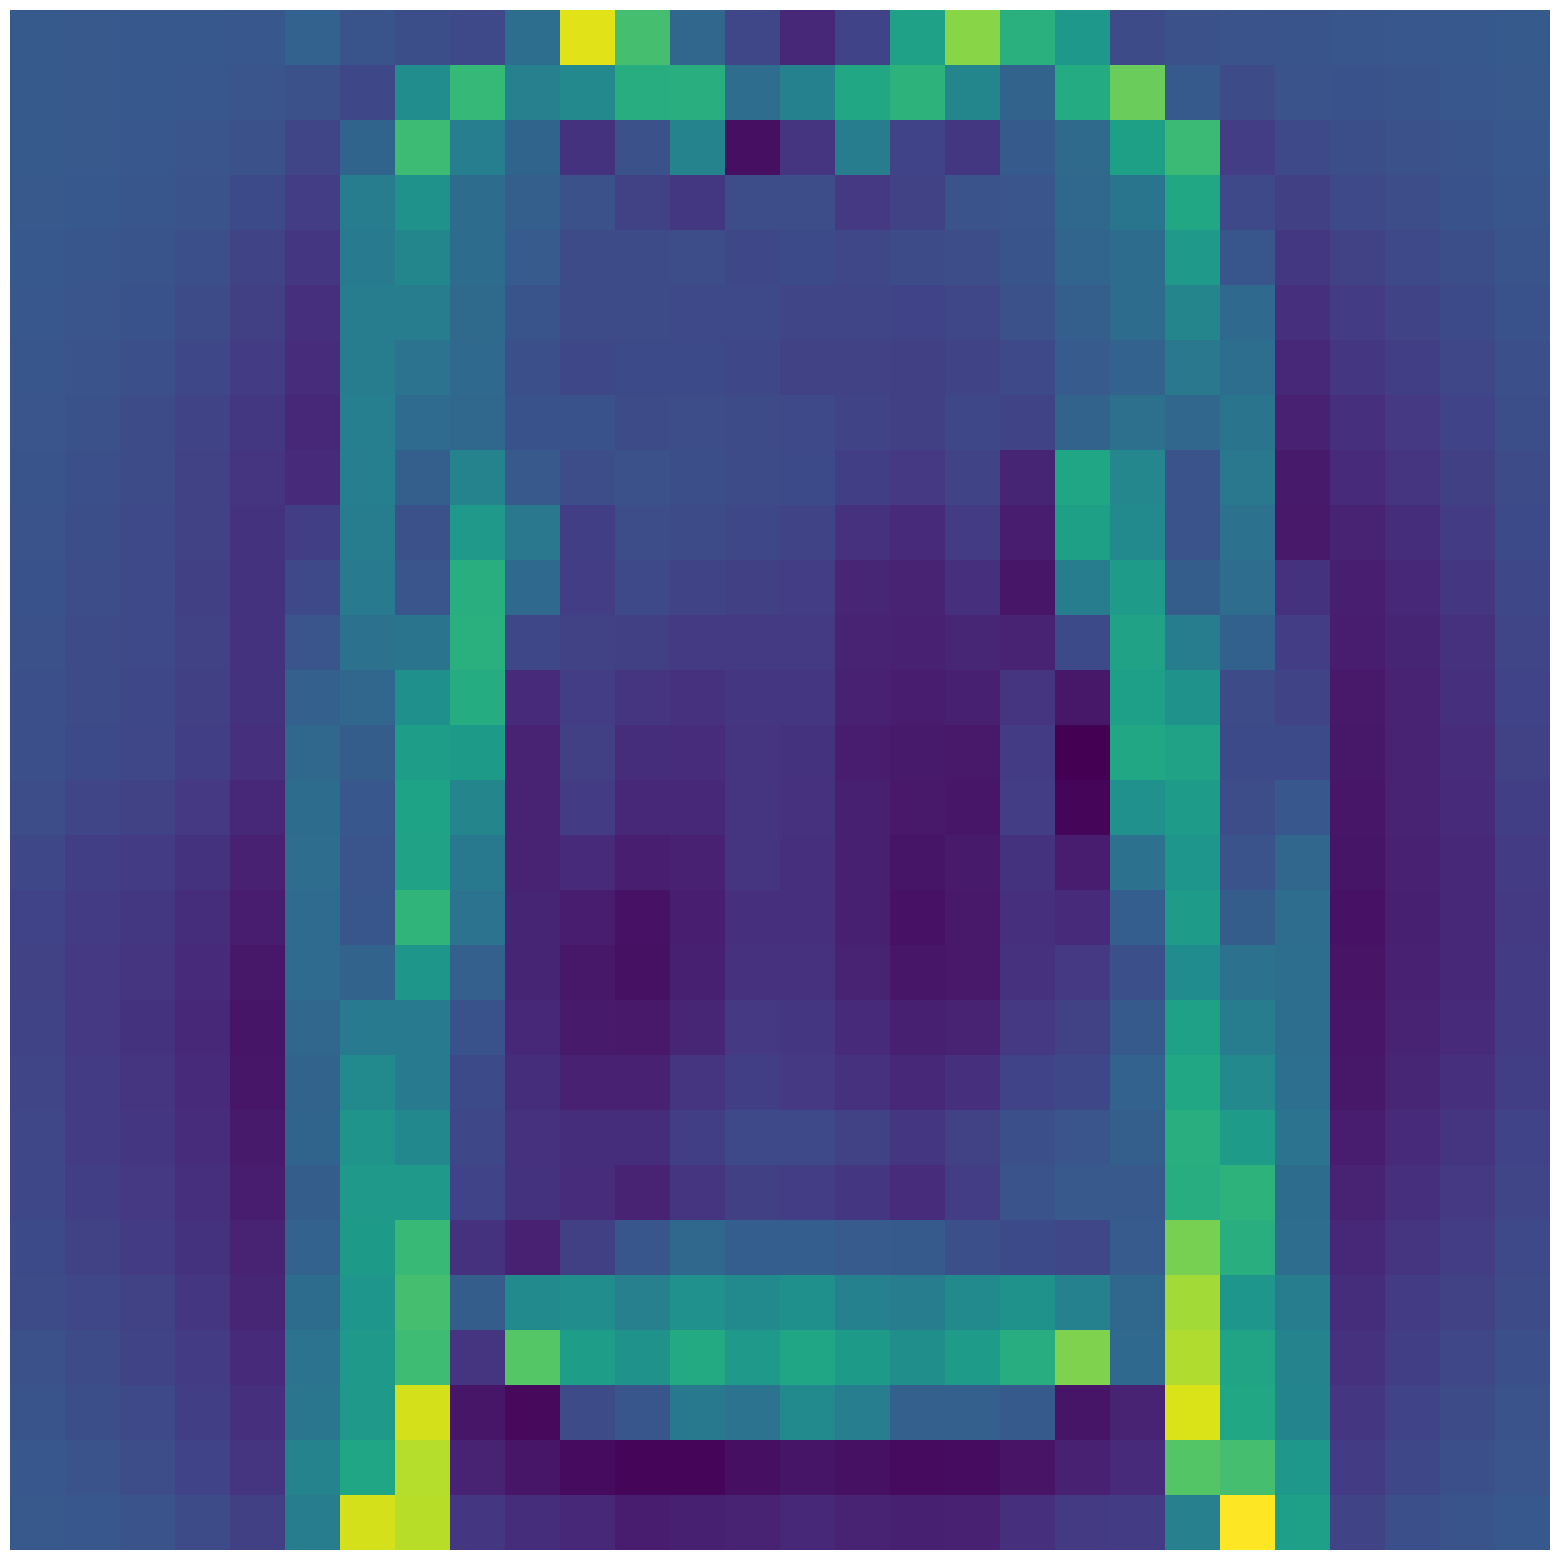
\includegraphics[width=0.35\linewidth]{figures/im.png} & 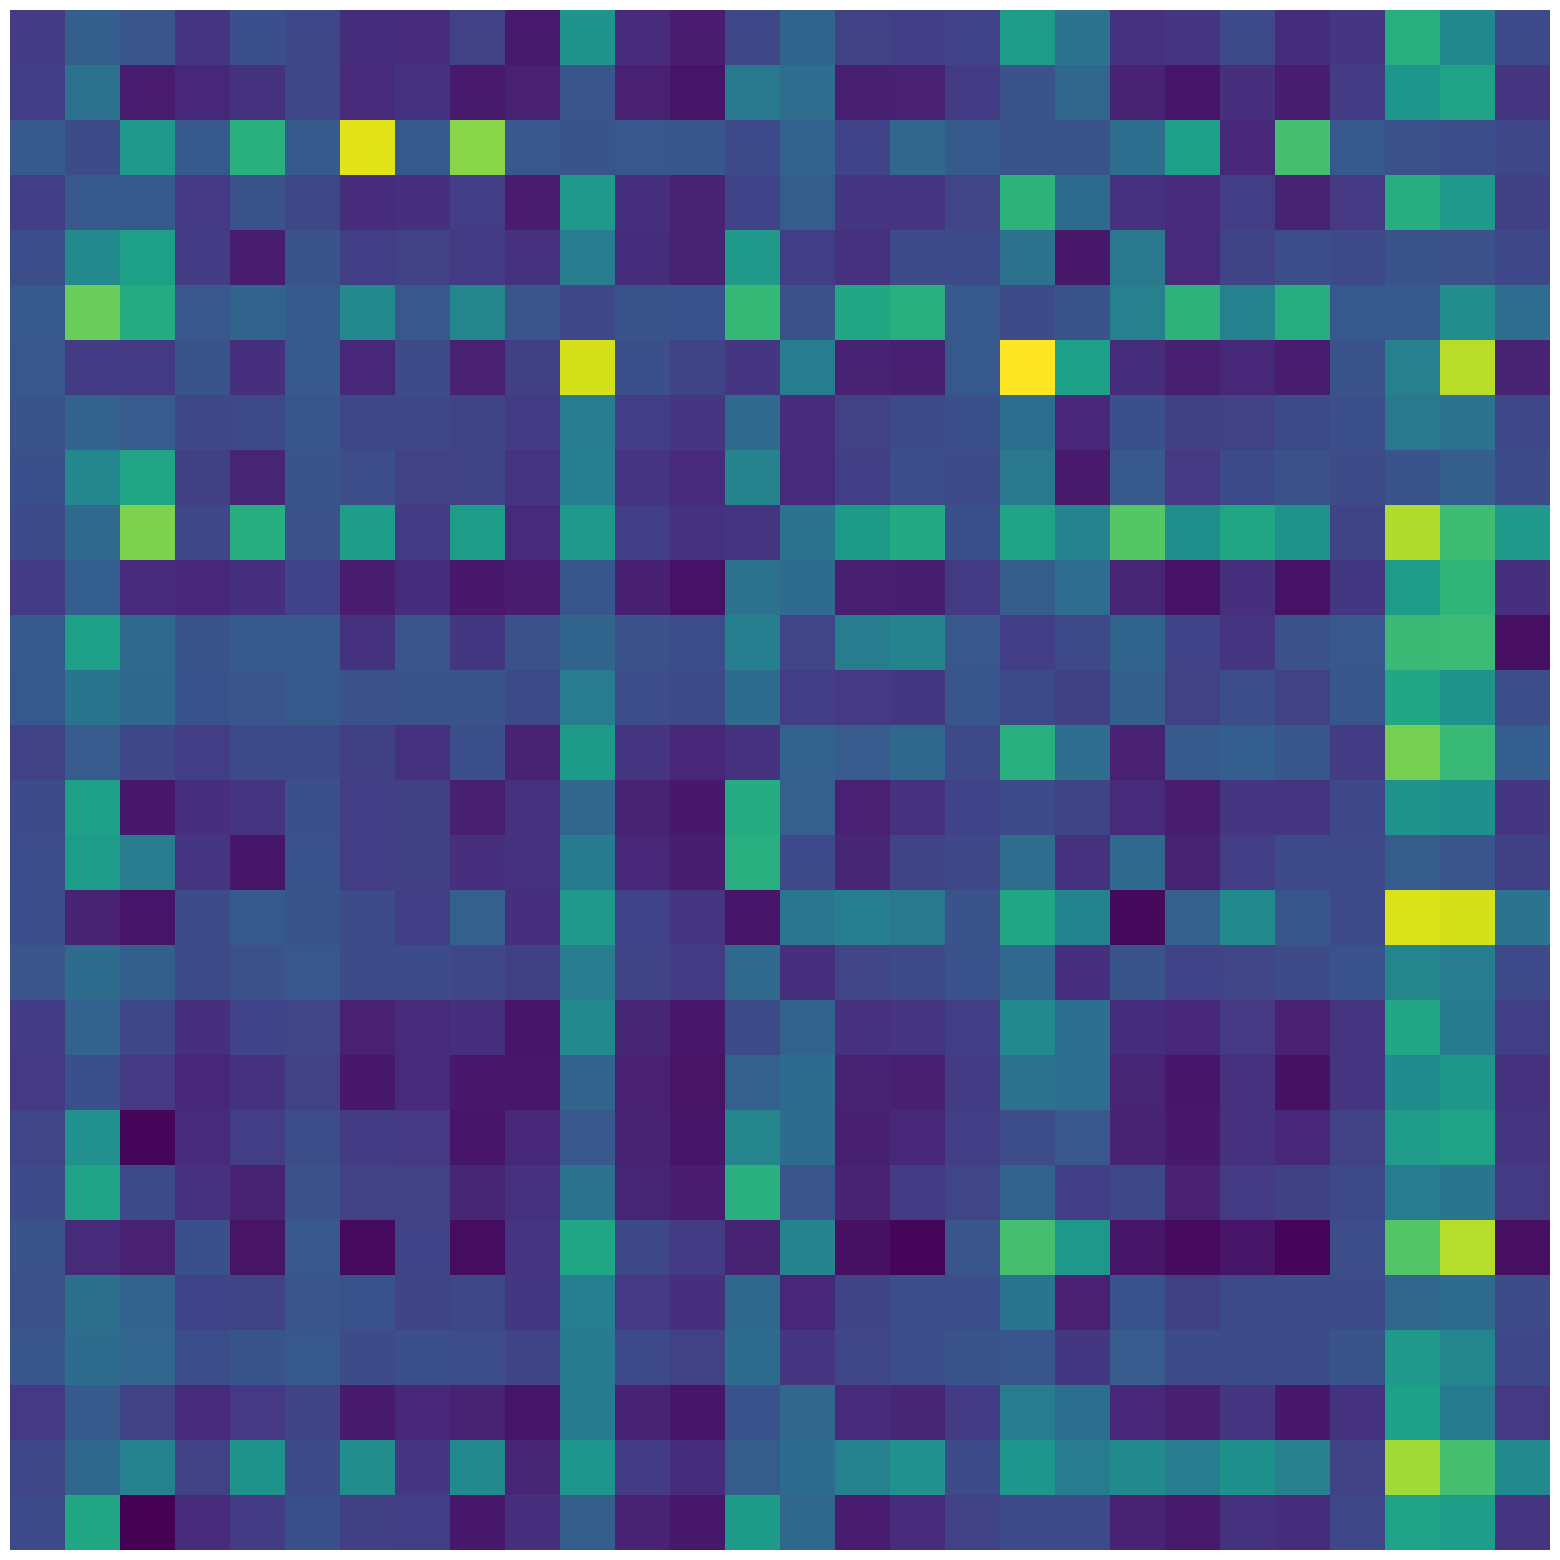
\includegraphics[width=0.35\linewidth]{figures/im_sort.png}
    \end{tabular}
  \end{center}
\end{frame}

\begin{frame}[fragile]
  \frametitle{2D Convolution}
  \begin{columns}
    \begin{column}{0.6\linewidth}
      \begin{itemize}
      \item Fully connected layer:
        \begin{align*}
          x^{(1)}_{pq} &=& \sigma\Bigg(\sum_{i,j=1}^{H,W}\mathbf{w}_{pqij}^{(0)}x_{ij}^{(0)} + b_{pq}^{(0)} \Bigg)
        \end{align*}

      \item Act locally: restrict to neighborhood of pixel \(p,q\)
        \begin{align*}
          x^{(1)}_{pq} &=& \sigma\Bigg(\sum_{i,j=-\Delta}^{i,j=+\Delta,}\mathbf{w}_{ij}^{(0)}x_{(p+i)(j+q)}^{(0)} + b^{(0)} \Bigg)
        \end{align*}
      \end{itemize}
    \end{column}
    \begin{column}{0.45\linewidth}
      \only<1>{
        \begin{center}
          \begin{tikzpicture}[>=stealth,thick,baseline]
            \matrix [matrix of math nodes,left delimiter=(,right delimiter=),ampersand replacement=\&, ](W){%
              w_{pq11} \& w_{pq12} \& \dots  \& w_{pq1j} \& \dots \& w_{pq1W}\\
              w_{pq21} \& w_{pq22} \& \dots  \& w_{pq2j} \& \dots \& w_{pq2W}\\  
              \vdots  \& \vdots  \&  \& \vdots  \&  \& \vdots\\
              w_{pqi1} \& w_{pqi2} \& \dots  \& w_{pqij} \& \dots \& w_{pqiW}\\
              \vdots  \& \vdots  \&  \& \vdots  \&  \& \vdots\\
              w_{pqH1} \& w_{pqH2} \& \dots  \& w_{pqHj} \& \dots \& w_{pqHW}\\
            };
          \end{tikzpicture}
        \end{center}
      }
      \only<2->{
        \begin{center}
          \begin{tikzpicture}[>=stealth,thick,baseline]
            \matrix [matrix of math nodes,left delimiter=(,right delimiter=),ampersand replacement=\&, ](W){%
              0 \& \dots  \& 0 \& \dots \& 0\\
              0 \& \dots  \& 0 \& \dots \& 0\\  
              \vdots  \&  w_{(i)(j-1)} \& w_{(i-1)(j)} \& w_{(i-1)(j+1)}   \& \vdots\\
              0 \& w_{(i)(j-1)} \& w_{(i)(j)} \& w_{(i)(j+1)} \& 0\\
              \vdots  \& w_{(i+1)(j-1)} \& w_{(i+1)(j)}  \& w_{(i+1)(j+1)} \& \vdots\\
              0 \& \dots  \& 0 \& \dots \& 0\\
            };
          \end{tikzpicture}
        \end{center}
      }
      \visible<4>{
        \begin{work}
          Show that 2D convolution can be expressed as a linear layer.
        \end{work}
      }
    \end{column}
  \end{columns}
\end{frame}

\begin{frame}
  \frametitle{Basics on 2D Convolution 1/2}
  \begin{center}
    \only<1>{%
      \centerline{\textbf{Convolution}}
      \begin{tikzpicture}[, %
        arr/.style={matrix of nodes,  ampersand replacement=\&,
          row sep=-\pgflinewidth, column sep=-\pgflinewidth,
          nodes={draw, minimum size=0.75cm}, font =\small}
        ]          
        \matrix[arr, ] (X) {
          |[fill=blue!50]| 0\&            |[fill=blue!50]|1\& |[fill=blue!50]|2\&3\&4\\
          |[fill=blue!50]|5\&            |[fill=blue!50]|6\&            |[fill=blue!50]|7\&8\&9\\
          |[fill=blue!50]|            10\&            |[fill=blue!50]|11\&            |[fill=blue!50]|12\&13\&14\\
          15\&16\&17\&18\&19\\
        };
        \node (*) [right = 0.2em of X] (m) {$*$};
        \matrix[arr, right = 0.2em of m] (K) {
          1 \& 1 \& 1 \\
          1 \& 1 \& 1 \\
          1 \& 1 \& 1 \\
        };
        \node (*) [right = 0.2em of K] (e) {$=$};
        \matrix[arr, right = 0.2em  of e] (Y) {
          |[fill=blue!50]|54 \& 63 \& 72 \\
          99 \& 108 \& 117 \\
        };
        \node (*) [below = of K] (k) {$K$};
        \node (*) [left = 3cm of k] {$X^{(h)}$};
        \node (*) [right = 2.5 cm of k] {$X^{(h+1)}$};
      \end{tikzpicture}
      
      {\small (More \url{https://github.com/vdumoulin/conv_arithmetic/blob/master/README.md})}
    }
    \only<2>{%
      \centerline{\textbf{Convolution + Padding (1,1)}}
      \begin{tikzpicture}[, %
        arr/.style={matrix of nodes,  ampersand replacement=\&,
          row sep=-\pgflinewidth, column sep=-\pgflinewidth,
          nodes={draw, minimum size=0.75cm}, font =\small}
        ]          
        \matrix[arr, ] (X) {
          |[fill=blue!50]| 0 \& |[fill=blue!50]| 0 \& |[fill=blue!50]| 0 \&0\& 0\& 0 \& 0\\
          |[fill=blue!50]| 0 \& |[fill=blue!50]| 0 \& |[fill=blue!50]|1\& 2\&3\&4 \& 0\\
          |[fill=blue!50]| 0 \& |[fill=blue!50]| 5 \& |[fill=blue!50]|6\& 7\&8\&9 \& 0\\
          0 \&         10\&         11\&     12\&13\&14 \& 0\\
          0 \& 15\&16\&17\&18\&19 \& 0\\
          0 \& 0 \&0 \&0\& 0\& 0 \& 0 \\
        };
        \node (*) [right = 0.2em of X] (m) {$*$};
        \matrix[arr, right = 0.2em of m] (K) {
          1 \& 1 \& 1 \\
          1 \& 1 \& 1 \\
          1 \& 1 \& 1 \\
        };
        \node (*) [right = 0.2em of K] (e) {$=$};
        \matrix[arr, right = 0.2em  of e] (Y) {
          |[fill=blue!50]| 12\&  21\&  27 \&  33\&  24\\
          33\&  54\&  63 \&  72\&  51\\
          63\&  99\& 108 \& 117\&  81\\
          52\&  81\&  87 \&  93\&  64\\
        };
      \end{tikzpicture}          
    }
    \only<3>{%
      \centerline{\textbf{Convolution + Padding (1,1) + Stride (3, 2)}}
      \begin{tikzpicture}[, %
        arr/.style={matrix of nodes,  ampersand replacement=\&,
          row sep=-\pgflinewidth, column sep=-\pgflinewidth,
          nodes={draw, minimum size=0.75cm}, font =\small}
        ]          
        \matrix[arr, ] (X) {
          |[fill=blue!50]| 0 \& |[fill=blue!50]| 0 \& |[fill=blue!50]| 0 \&0\& 0\& 0 \& 0\\
          |[fill=blue!50]| 0 \& |[fill=blue!50]| 0 \& |[fill=blue!50]|1\& 2\&3\&4 \& 0\\
          |[fill=blue!50]| 0 \& |[fill=blue!50]| 5 \& |[fill=blue!50]|6\& 7\&8\&9 \& 0\\
          0 \&         10\&            11\&       12\&13\&14 \& 0\\
          0 \& 15\&16\&17\&18\&19 \& 0\\
          0 \& 0 \&0 \&0\& 0\& 0 \& 0 \\
        };
        \node (*) [right = 0.2em of X] (m) {$*$};
        \matrix[arr, right = 0.2em of m] (K) {
          1 \& 1 \& 1 \\
          1 \& 1 \& 1 \\
          1 \& 1 \& 1 \\
        };
        \node (*) [right = 0.2em of K] (e) {$=$};
        \matrix[arr, right = 0.2em  of e] (Y) {
          |[fill=blue!50]| 12\&   27 \&   24\\
          52\&   87 \&   64\\
        };
      \end{tikzpicture}          
    }
    
    \only<4>{%
      \centerline{\textbf{Convolution for multivalued images}}
      \begin{tikzpicture}[, %
        arr/.style={matrix of nodes,  ampersand replacement=\&,
          row sep=-\pgflinewidth, column sep=-\pgflinewidth,
          nodes={draw, minimum size=0.75cm}, font =\small}
        ]          
        \matrix[arr, ] (X1) {
          |[fill=blue!50]| 0\&            |[fill=blue!50]|1\& |[fill=blue!50]|2\&3\&4\\
          |[fill=blue!50]|5\&            |[fill=blue!50]|6\&            |[fill=blue!50]|7\&8\&9\\
          |[fill=blue!50]|            10\&            |[fill=blue!50]|11\&            |[fill=blue!50]|12\&13\&14\\
          15\&16\&17\&18\&19\\
        };
        \node (*) [right = 0.2em of X1] (m1) {$*$};
        \matrix[arr, right = 0.2em of m1] (K1) {
          1 \& 1 \& 1 \\
          1 \& 1 \& 1 \\
          1 \& 1 \& 1 \\
        };
        \node (*) [right = 0.2em of K1] (e1) {$=$};
        \matrix[arr, right = 0.2em  of e1] (Y1) {
          |[fill=blue!50]|54 \& 63 \& 72 \\
          99 \& 108 \& 117 \\
        };
        
        \matrix[arr, below = 0.5cm of X1] (X2) {
          |[fill=blue!50]| 19\&            |[fill=blue!50]|18\& |[fill=blue!50]|17\& 16\& 15\\
          |[fill=blue!50]| 14\&            |[fill=blue!50]|13\& |[fill=blue!50]|12 \& 11\&10\\
          |[fill=blue!50]| 9\&            |[fill=blue!50]|8\& |[fill=blue!50]|7\&6\&5\\
          4\&3\&2\&1\&0\\
        };
        \node (*) [right = 0.2em of X2] (m2) {$*$};
        \matrix[arr, right = 0.2em of m2] (K2) {
          2 \& 2 \& 2 \\
          2 \& 2 \& 2 \\
          2 \& 2 \& 2 \\
        };
        \node (*) [right = 0.2em of K2] (e2) {$=$};
        \matrix[arr, right = 0.2em  of e2] (Y2) {
          |[fill=blue!50]|234 \& 216 \& 198 \\
          144 \& 126 \& 108 \\
        };
        \node (*) [below= 0.75cm  of Y1](p) {$+$};
        \node (*) [right = of p] (e3){$=$};
        \matrix[arr, right = 0.2em  of e3] (Y2) {
          |[fill=blue!50]| 288 \& 279 \& 270\\
          243 \& 234 \& 225\\
        };        
      \end{tikzpicture}
    }
  \end{center}
\end{frame}

\begin{frame}
  \frametitle{Basics of 2D Convolution 2/2}
  \begin{itemize}
  \item Multivariate input - Multivariate output
    \begin{align*}
      \mathbf{X}^{(h)} & \in {} \mathbb{R}^{C_{(h)} \times H^{(h)} \times W^{(h)}}\\
      \mathbf{K}^{(h)} & \in {} \mathbb{R}^{C_{(h+1)}\times C_{(h)} \times k_{H}^h \times k_{W}^h}\\
      \mathbf{X}^{(h+1)}& \in {} \mathbb{R}^{C_{(h+1)} \times H^{(h+1)} \times W^{(h+1)}}\\
    \end{align*}
  \item Special case of \(1\times 1\) convolution: \((C_{(h+1)}, C_{(h)}, k_H, K_W) = (C_o, C_i,1,1)\)
    \begin{itemize}
      \item Combine pixel across channels - no spatial operation
      \item Matrix product / linear layer in the channel dimension
    \begin{align*}
      \mathbf{X}^{(h+1)} = \reshape\bigg\{\sigma\big(\mathbf{K}^{(h)}\reshape\big\{\mathbf{X}^{(h)}, C_{(h)}, H^{(h)}W^{(h)}\big\}+\mathbf{b}^{(h)}\big), C_{(h+1)}, H^{(h)},W^{(h)}\bigg\}
    \end{align*}
    with \(\reshape\big\{\mathbf{X}^{(h)}, C_{(h)}, H^{(h)}W^{(h)}\big\}\in\mathbb{R}^{C_{(h)}\times H^{(h)}W^{(h)}}\)
      
    \end{itemize}
  \end{itemize}
\end{frame}

\begin{frame}
  \frametitle{Pooling}
  \begin{itemize}
  \item Reduce the resolution of the image \(\equiv\) Use larger convolution kernel
  \item Downsampling with simple operator on the neighborhood:
    \begin{itemize}
    \item Average value
    \item Max value (preferred)
    \end{itemize}
  \item After the non-linearity
  \end{itemize}
  \begin{center}
    \begin{tikzpicture}[%
        arr/.style={matrix of nodes,  ampersand replacement=\&,
          row sep=-\pgflinewidth, column sep=-\pgflinewidth,
          nodes={draw, minimum size=0.75cm}, font =\small}
        ]          
        \matrix[arr, ] (X) {
          |[fill=blue!50]| 0\&            |[fill=blue!50]|1\& 2\&3\&4\\
          |[fill=blue!50]|5\&            |[fill=blue!50]|6\& 7\&8\&9\\
          10\&            11\&            12\&13\&14\\
          15\&16\&17\&18\&19\\
        };
        \node[right = of X, draw, align=left] (mp) {\(2\times 2\) MaxPooling \\ Stride=2};
        \matrix[arr, right = of mp ] (Xp) {
          |[fill=blue!50]| 6\&   8\\
          16 \& 18 \\
        };      
        
      \end{tikzpicture}
    \end{center}
  \end{frame}

  \begin{frame}{2D CNN}
    \begin{work}
      \begin{itemize}
      \item Express multi-channels \& multi-outputs convolution as a matrix product.
      \item Show that the successive convolution with two kernels is equivalent to one convolution.
      \item What stride size wiil you use for a max pooling with a kernel of size \(2 \times 2\)?
      \item Implement a CNN for the classification of \emph{Fashion MNIST} data set: use one or two convolutional layers for the MLP.
      \end{itemize}
    \end{work}    
  \end{frame}

  \subsection{How to improve the learning process}

  \begin{frame}
    \frametitle{Batch Normalization}
    \begin{itemize}
    \item Remember scaling problem in slide \ref{scale_frame}
    \item Similar problem may happen to each layer \textbf{but} we cannot use the same trick: the sample mean/variance change after each batch update !
    \item<2-> Apply normalization per batch: \emph{Batch Normalization}
      \begin{align*}
        \tilde{\mathbf{x}}_B = \boldsymbol{\gamma}\odot\Big[(\mathbf{x}_B-\boldsymbol{\mu}_B)\oslash\boldsymbol{\sigma}_B\Big] + \boldsymbol{\beta}
      \end{align*}
      with \(\boldsymbol{\mu}_B\) and \(\boldsymbol{\sigma}_B\) computed on batch \(B\), and \(\boldsymbol{\gamma} \& \boldsymbol{\beta}\) are learnable parameters
    \end{itemize}

    \visible<3>{
      \begin{work}
        \begin{itemize}
        \item What happen if the batch size is one ?
        \item What happen if the batch size is small ?
        \item What should we do in \emph{prediction} mode ?
        \item Add normalization layer (2D) to your model.
        \end{itemize}
      \end{work}
    }
  \end{frame}

  \begin{frame}{Data Augmentation}
    \begin{itemize}
    \item Noise injection to generate / augment data set: \((\mathbf{x}, y) \rightarrow (\tilde{\mathbf{x}}, y)\)
    \item For image classification it is \emph{relatively} easy:
      \begin{itemize}
      \item Geometric tansformation: Rotation, translation, symmetry, radiometry \ldots
      \item Radiometric transformation: Invert, jitter \ldots
      \item \emph{Any transformation that can model the variability of the acquisition process}
      \end{itemize}
    \end{itemize}
  
  \begin{center}
    \begin{tabular}{c@{~}c@{~}c@{~}c@{~}c}
      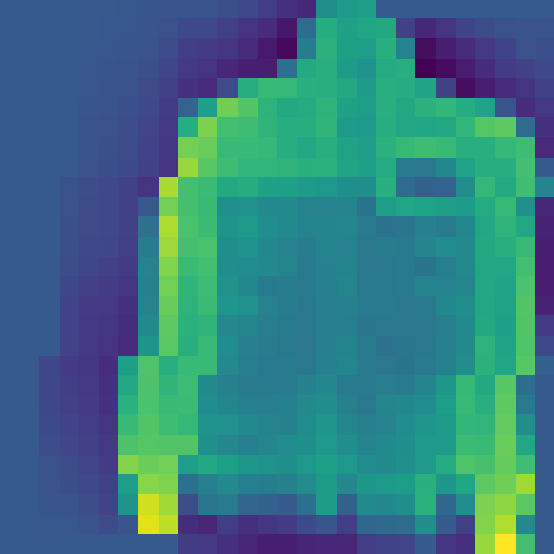
\includegraphics[width=0.2\linewidth]{figures/data_augment_0.pdf}&         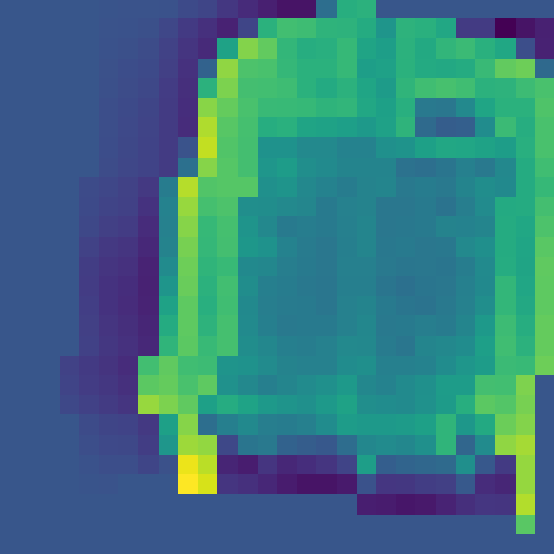
\includegraphics[width=0.2\linewidth]{figures/data_augment_1.pdf}&        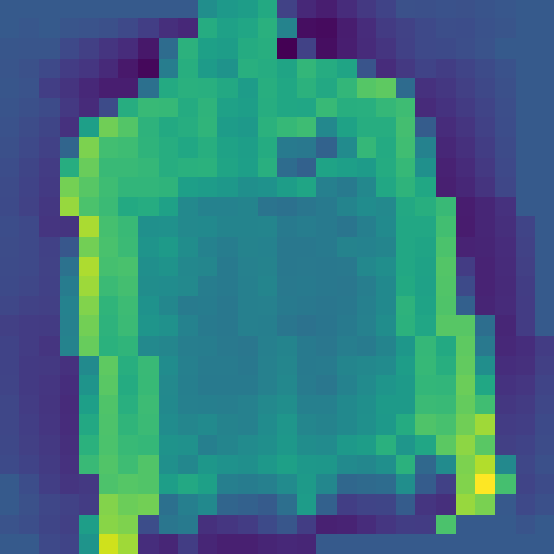
\includegraphics[width=0.2\linewidth]{figures/data_augment_2.pdf}&        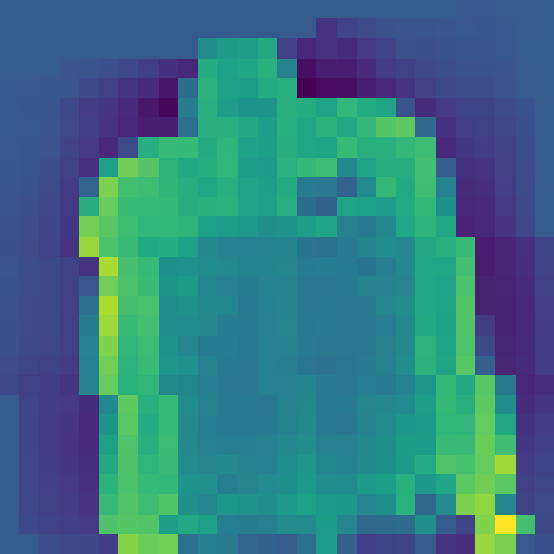
\includegraphics[width=0.2\linewidth]{figures/data_augment_3.pdf}&        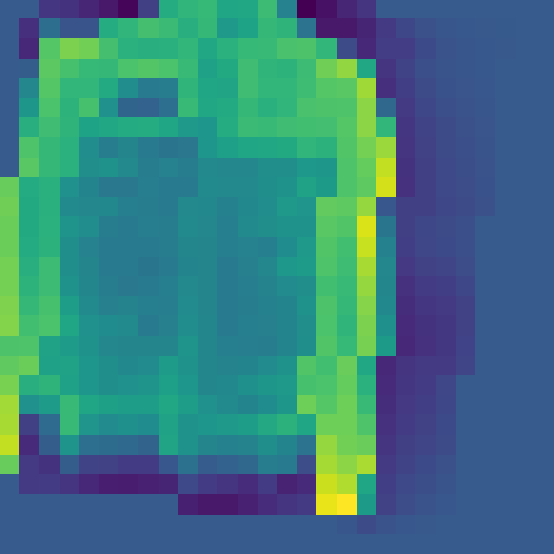
\includegraphics[width=0.2\linewidth]{figures/data_augment_4.pdf}
    \end{tabular}
  \end{center}
 
    \begin{work}
      Implement data augmentation with Pytorch for the training data only.
    \end{work}
  \end{frame}

  \begin{frame}
    \frametitle{Residual Network}
    \begin{itemize}
    \item Deep Neural Network: \(f_h(\mathbf{x}^{(h)}) := f_h(\mathbf{x}^{(h)}, \theta_h)\)
      \[f(\mathbf{x}) = f_H\circ f_{H-1}\circ \ldots \circ f_0(\mathbf{x})\]
\only<2>{\item Let \(f_h = g_2\circ g_1\circ g_0\)
      \begin{center}
        \begin{tikzpicture}
          \node (x) at (0,0) {\(\mathbf{x}\)};
          \node[right= of x] (x1) {\(\mathbf{x}^{(1)}\)};
          \node[right= of x1] (x2) {\(\mathbf{x}^{(2)}\)};
          \node[right= of x2] (y) {\(f_h(\mathbf{x})\)};
          \path [->] (x) edge node[above] {$g_0$} (x1);
          \path [->] (x1) edge node[above] {$g_1$} (x2);
          \path [->] (x2) edge node[above] {$g_2$} (y);
        \end{tikzpicture}
      \end{center}
      \begin{align*}
        \dfrac{\partial f_h(\mathbf{x})}{\partial \alpha_0} = \underrightarrow{\dfrac{g_2}{g_1}\circ\dfrac{g_1}{g_0}\circ\dfrac{g_0}{\alpha_0}(\mathbf{x})} \qquad         \dfrac{\partial g(\mathbf{x})}{\partial \alpha_1} = \dfrac{g_2}{g_1}\circ\dfrac{g_1}{\alpha_1}(\mathbf{x}^{(1)}) \qquad  \dfrac{\partial g(\mathbf{x})}{\partial \alpha_2} = \dfrac{g_2}{\alpha_2}(\mathbf{x}^{(2)})
      \end{align*}}
  \only<3>{\item Let \(f_h = g_2\circ g_1\circ g_0\) with \emph{residual connection}
      \begin{center}
    \begin{tikzpicture}
      \node (x) at (0,0) {\(\mathbf{x}\)};
      \node[right= of x] (p1) {\(\oplus \)};
      \node[right= 0.25cm of p1] (x1) {\(\mathbf{x}^{(1)}\)};
      
      \node[right= of x1] (p2) {\(\oplus\)};
      \node[right= 0.25cm of p2] (x2) {\(\mathbf{x}^{(2)}\)};

      \node[right= of x2] (p3) {\(\oplus\)};
      \node[right= 0.25cm of p3] (y) {\(f_h(\mathbf{x})\)};
      % \node[right= of x2] (y) {\(y\)};
      
      
      \path [->] (x) edge node[above] {$g_0$} (p1);
      \path[->] (p1) edge node{} (x1);
      \path[->] (x) edge [bend right]  node {} (p1);
      
      \path [->] (x1) edge node[above] {$g_1$} (p2);
      \path[->] (p2) edge node{} (x2);
      \path[->] (x1) edge [bend right]  node {} (p2);

      
      \path [->] (x2) edge node[above] {$g_2$} (p3);
      \path[->] (p3) edge node{} (y);
      \path[->] (x2) edge [bend right]  node {} (p3);
      
    \end{tikzpicture}
  \end{center}
  \begin{align*}
    \dfrac{\partial f_h(\mathbf{x})}{\partial \alpha_0} = \dfrac{g_2}{g_1}\circ\dfrac{g_1}{g_0}\circ\dfrac{g_0}{\alpha_0}(\mathbf{x}) + \dfrac{g_1}{g_0}\circ\dfrac{g_0}{\alpha_0}(\mathbf{x}) + \dfrac{g_0}{\alpha_0}(\mathbf{x}) 
  \end{align*}
  \begin{itemize}
  \item Improve gradient propagation
  \item Prevent vanishing/shattered gradient
  \end{itemize}
}
\end{itemize}
\only<4>{%
  \centerline{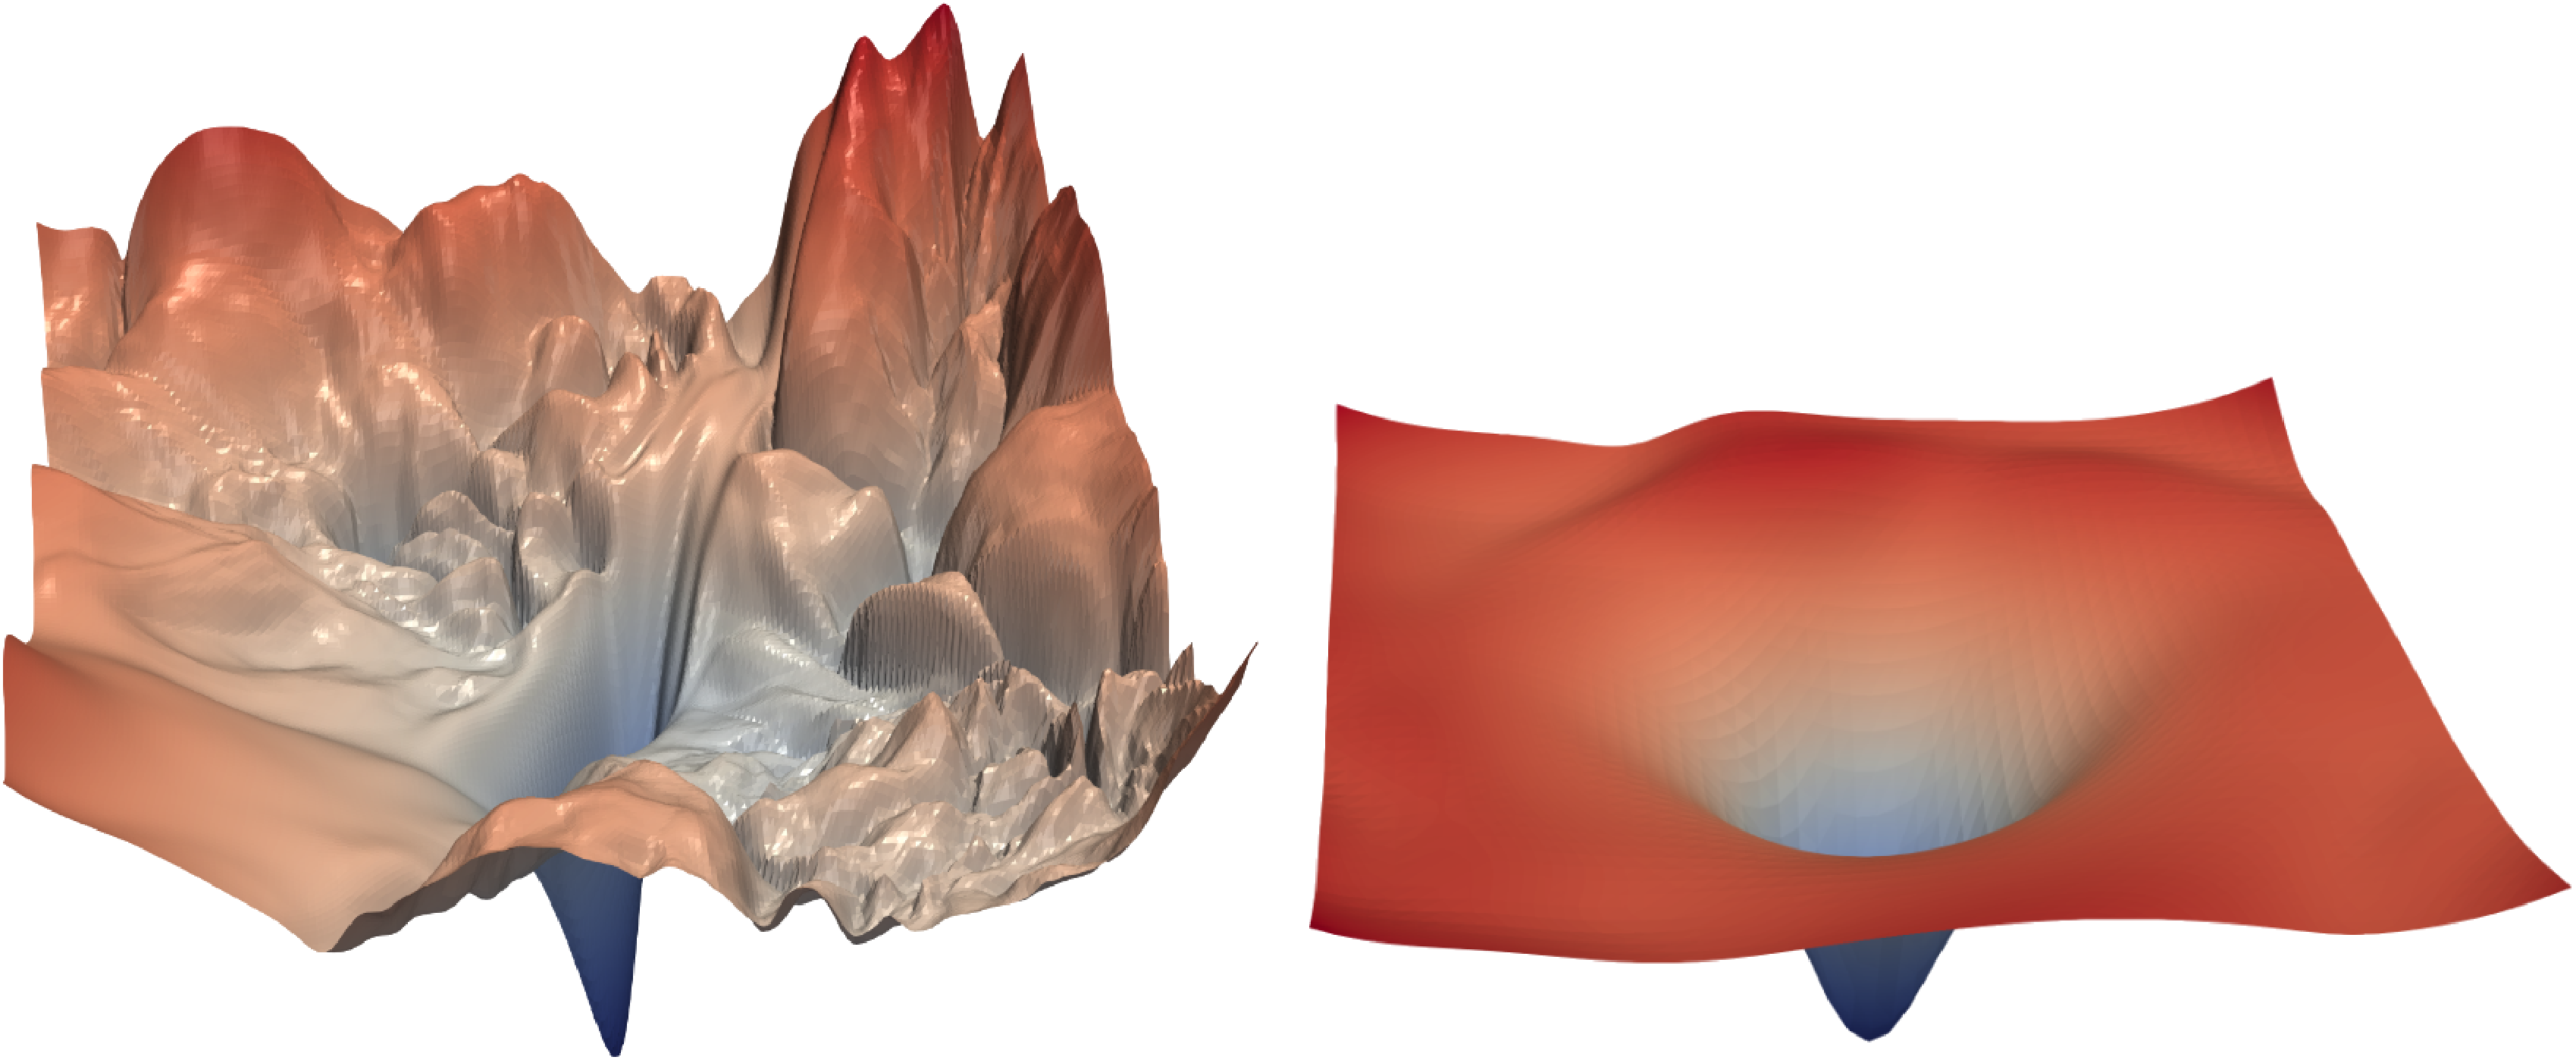
\includegraphics[width=0.75\linewidth]{figures/loss_landscape.pdf}}

  {\small From \cite{10.5555/3327345.3327535}}
}
\end{frame}

\section{Recurrent Neural Networks}

\subsection{When order matters}
\begin{frame}
  \frametitle{Sequential data}

  \begin{itemize}
  \item Time series
    \begin{center}
      \begin{tikzpicture}
        \begin{axis}[domain=0:10, samples=200, grid, very thick, footnotesize, ymin=-1.0, ymax=1.0, xmin=0, xmax=15, width=0.5\linewidth, height=0.25\linewidth]
          \addplot[red] {sin(deg(x))*exp(-x/10) + 0.1*rnd};
          \addplot[blue, domain=10:15, dashed] {sin(deg(x))*exp(-x/10)};
        \end{axis}
      \end{tikzpicture}
    \end{center}
  \item Text data
    \begin{center}
      \Large
      \textcolor{red}{This course is really} \textcolor{blue}{cool}
    \end{center}
  \end{itemize}
\end{frame}


\begin{frame}{Auto-regressive model}
  \begin{itemize}
  \item Autogressive models: \(p(\mathbf{x}_t | \mathbf{x}_{t-1}, \ldots, \mathbf{x}_1)\)
  \item Sequence model:
    \[p(\mathbf{x}_T , \mathbf{x}_{T-1}, \ldots, \mathbf{x}_1) = \prod_{t=2}^{T}p(\mathbf{x}_t | \mathbf{x}_{t-1}, \ldots, \mathbf{x}_1)p(\mathbf{x}_1) \]
  \item Markov model:
    \[p(\mathbf{x}_T | \mathbf{x}_{T-1}, \ldots, \mathbf{x}_1) = \prod_{t=2}^{T}p(\mathbf{x}_t |\mathbf{x}_{t-1}) p(\mathbf{x}_1)\]
  \item <2> Example: \(p(\mathbf{x}_t |\mathbf{x}_{t-1})\) could model
    \begin{itemize}
    \item The probability to get letter after a observing a specific letter (or a set of)
    \item The expected value of a signal given past values of the same signal
    \end{itemize}
    
  \end{itemize}
  
\end{frame}

% \begin{frame}
%   \frametitle{Main sequence models}
%   \begin{center}
%     \begin{tikzpicture}[=>latex]
%       \node (x0) [] {\(x_0\)};
%       \node (x1) [right of=x0] {\(x_1\)};
%       \node (x2) [right of=x1] {\(x_2\)};     
%       \node (h0) [above of=x0] {\(h_0\)};
%       \node (h1) [right of=h0] {\(h_1\)};
%       \node (h2) [right of=h1] {\(h_2\)};
%       \node (o) [above of=h0] {\(o\)};
%     \end{tikzpicture}
%   \end{center}
% \end{frame}


\begin{frame}{Latent autoregressive model}
  \begin{columns}
    \begin{column}{0.55\linewidth}
      \begin{center}
        \begin{tikzpicture}[=>latex, node distance=2cm]
          \node[rectangle, draw=black, fill=blue!50, minimum size=0.75cm] (x0) [ ] {\(\mathbf{x}_{t-1}\)};
          \node[rectangle, draw=black, fill=blue!50, minimum size=0.75cm] (x1) [right of=x0] {\(\mathbf{x}_{t}\)};
          \node[rectangle, draw=black, fill=blue!50, minimum size=0.75cm] (x2) [right of=x1] {\(\mathbf{x}_{t+1}\)};     
          \node[rectangle, draw=black, fill=blue!50, minimum size=0.75cm] (h0) [above of=x0] {\(\mathbf{h}_{t-1}\)};
          \node[rectangle, draw=black, fill=blue!50, minimum size=0.75cm] (h1) [right of=h0] {\(\mathbf{h}_{t}\)};
          \node[rectangle, draw=black, fill=blue!50, minimum size=0.75cm] (h2) [right of=h1] {\(\mathbf{h}_{t+1}\)};
          \node[rectangle, draw=black, fill=blue!50, minimum size=0.75cm] (o0) [above of=h0] {\(\mathbf{o}_{t-1}\)};
          \node[rectangle, draw=black, fill=blue!50, minimum size=0.75cm] (o1) [right of=o0] {\(\mathbf{o}_{t}\)};
          \node[rectangle, draw=black, fill=blue!50, minimum size=0.75cm] (o2) [right of=o1] {\(\mathbf{o}_{t+1}\)};

          \node[] (hp) [left of=h0] {};
          \node[] (hf) [right of=h2] {};
          
          \draw[->] (h0)--(h1);
          \draw[->] (h1)--(h2);
          \draw[->] (x0)--(h0);
          \draw[->] (x1)--(h1);
          \draw[->] (x2)--(h2);
          \draw[->] (h0)--(o0);
          \draw[->] (h1)--(o1);
          \draw[->] (h2)--(o2);
          \draw[->, dashed] (hp)--(h0);
          \draw[->, dashed] (h2)--(hf);
        \end{tikzpicture}
      \end{center}
    \end{column}
    \begin{column}{0.5\linewidth}
      \begin{itemize}
      \item \(\mathbf{h}_t = f(\mathbf{x}_{t}, \mathbf{h}_{t-1}) = \sigma_{h}\big(\mathbf{W}_{hx}\mathbf{x}_{t} + \mathbf{W}_{hh}\mathbf{h}_{t-1} + \mathbf{b}_h\big)\)
      \item \(\mathbf{o}_t = g(\mathbf{h}_{t}) = \sigma_{o}\big(\mathbf{W}_{oh}\mathbf{h}_t+\mathbf{b}_o\big)\)
      \item Backpropagation through time - BPTT
        \[\ell = \frac{1}{T}\sum_{t=1}^T\ell(\mathbf{y}_{t}, {\mathbf{o}}_{t})\]
        with \(\mathbf{h}_{0}= \mathbf{0}\)
      \end{itemize}
      
    \end{column}
  \end{columns}
\end{frame}

\begin{frame}
  \frametitle{Issue with BPTT}
  \begin{align*}
    \frac{\partial \ell}{\partial \mathbf{W}_{hh}} =&    \frac{1}{T}\sum_{t=1}^T\frac{\partial \ell(\mathbf{y}_{t}, {\mathbf{o}}_{t})}{\partial \mathbf{W}_{hh}} \\
    =&  \frac{1}{T}\sum_{t=1}^T\frac{\partial \ell(\mathbf{y}_{t}, {\mathbf{o}}_{t})}{\partial {\mathbf{o}}_{t}}\frac{\partial{\mathbf{o}}_{t}}{\partial \mathbf{W}_{hh}} \\
    =&  \frac{1}{T}\sum_{t=1}^T\frac{\partial \ell(\mathbf{y}_{t}, {\mathbf{o}}_{t})}{\partial {\mathbf{o}}_{t}}\frac{\partial g(\mathbf{h}_{t})}{\partial\mathbf{h}_t}\bigg[\frac{\partial f(\mathbf{x}_{t}, \mathbf{h}_{t-1})}{\partial \mathbf{W}_{hh}} + \frac{f(\mathbf{x}_{t}, \mathbf{h}_{t-1})}{\partial\mathbf{h}_{t-1}}\frac{\partial \mathbf{h}_{t-1}}{\partial \mathbf{W}_{hh}}\bigg]\\
    =&  \frac{1}{T}\sum_{t=1}^T\frac{\partial \ell(\mathbf{y}_{t}, {\mathbf{o}}_{t})}{\partial {\mathbf{o}}_{t}}\frac{\partial g(\mathbf{h}_{t})}{\partial\mathbf{h}_t}\Bigg[\frac{\partial f(\mathbf{x}_{t}, \mathbf{h}_{t-1})}{\partial \mathbf{W}_{hh}} +  \textcolor{blue}{ \sum_{p=1}^{t-1}\bigg(\prod_{q=p+1}^{t} \frac{\partial f(\mathbf{x}_{q}, \mathbf{h}_{q-1})}{\partial \mathbf{h}_{q-1}} \bigg) \frac{\partial f(\mathbf{x}_{p}, \mathbf{h}_{p-1})}{\partial \mathbf{W}_{hh}}}\Bigg]\\
  \end{align*}
  
\end{frame}

\subsection{Modern RNN}

\begin{frame}[fragile]
  \frametitle{Long Short Term Memory  (LSTM)}
  \begin{columns}
    \begin{column}{0.65\linewidth}
      \newcommand{\empt}[2]{$\mathbf{#1}^{(#2)}$}
      
      \begin{tikzpicture}[
        % GLOBAL CFG
        font=\sf \scriptsize,
        >=LaTeX,
        % Styles
        cell/.style={% For the main box
          rectangle, 
          rounded corners=5mm, 
          draw,
          very thick,
        },
        operator/.style={%For operators like +  and  x
          circle,
          draw,
          inner sep=-0.5pt,
          minimum height =.5cm,
        },
        function/.style={%For functions
          ellipse,
          draw,
          inner sep=1pt
        },
        ct/.style={% For external inputs and outputs
          circle,
          draw,
          line width = .75pt,
          minimum width=1cm,
          inner sep=1pt,
        },
        gt/.style={% For internal inputs
          rectangle,
          draw,
          minimum width=4mm,
          minimum height=3mm,
          inner sep=1pt
        },
        mylabel/.style={% something new that I have learned
          font=\scriptsize\sffamily
        },
        ArrowC1/.style={% Arrows with rounded corners
          rounded corners=.25cm,
          thick,
        },
        ArrowC2/.style={% Arrows with big rounded corners
          rounded corners=.5cm,
          thick,
        },
        ]

        % Start drawing the thing...    
        % Draw the cell: 
        \node [cell, minimum height =4cm, minimum width=6cm] at (0,0){} ;

        % Draw inputs named ibox#
        \node [gt, label={[mylabel, shift={(0,0.25)}]left:\(\mathbf{F}_t\)}] (ibox1) at (-2,-0.75) {$\sigma$};
        \node [gt, label={[mylabel, shift={(0,0.25)}]right:\(\mathbf{I}_t\)}] (ibox2) at (-1.5,-0.75) {$\sigma$};
        \node [gt, minimum width=1cm, label={[mylabel, shift={(-0.125,0.25)}]right:\(\tilde{\mathbf{C}}_t\)}] (ibox3) at (-0.5,-0.75) {$\tanh$};
        \node [gt, label={[mylabel, shift={(0,0.25)}]right:\(\mathbf{O}_t\)}] (ibox4) at (0.5,-0.75) {$\sigma$};

        % Draw opérators   named mux# , add# and func#
        \node [operator] (mux1) at (-2,1.5) {$\times$};
        \node [operator] (add1) at (-0.5,1.5) {+};
        \node [operator] (mux2) at (-0.5,0) {$\times$};
        \node [operator] (mux3) at (1.5,0) {$\times$};
        \node [function] (func1) at (1.5,0.75) {$\tanh$};

        % Draw External inputs? named as basis c,h,x
        \node[ct] (c) at (-4,1.5) {\empt{c}{t-1}};
        \node[ct] (h) at (-4,-1.5) {\empt{h}{t-1}};
        \node[ct] (x) at (-2.5,-3) {\empt{x}{t}};

        % Draw External outputs? named as basis c2,h2,x2
        \node[ct] (c2) at (4,1.5) {\empt{c}{t}};
        \node[ct] (h2) at (4,-1.5) {\empt{h}{t}};
        % \node[ct, label={[mylabel]left:Label3}] (x2) at (2.5,3) {\empt{h}{t}};

        % Start connecting all.
        % Intersections and displacements are used. 
        % Drawing arrows    
        \draw [ArrowC1] (c) -- (mux1) -- (add1) -- (c2);

        % Inputs
        \draw [ArrowC2] (h) -| (ibox4);
        \draw [ArrowC1] (h -| ibox1)++(-0.5,0) -| (ibox1); 
        \draw [ArrowC1] (h -| ibox2)++(-0.5,0) -| (ibox2);
        \draw [ArrowC1] (h -| ibox3)++(-0.5,0) -| (ibox3);
        \draw [ArrowC1] (x) -- (x |- h)-| (ibox3);

        % Internal
        \draw [->, ArrowC2] (ibox1) -- (mux1);
        \draw [->, ArrowC2] (ibox2) |- (mux2);
        \draw [->, ArrowC2] (ibox3) -- (mux2);
        \draw [->, ArrowC2] (ibox4) |- (mux3);
        \draw [->, ArrowC2] (mux2) -- (add1);
        \draw [->, ArrowC1] (add1 -| func1)++(-0.5,0) -| (func1);
        \draw [->, ArrowC2] (func1) -- (mux3);

        % Outputs
        \draw [-, ArrowC2] (mux3) |- (h2);
        % \draw (c2 -| x2) ++(0,-0.1) coordinate (i1);
        % \draw [-, ArrowC2] (h2 -| x2)++(-0.5,0) -| (i1);
        % \draw [-, ArrowC2] (i1)++(0,0.2) -- (x2);

      \end{tikzpicture}
    \end{column}
    \begin{column}{0.375\linewidth}
      \begin{itemize}
      \item Forget gate
        \[\mathbf{F}_t = \sigma\Big(\textcolor{blue}{\mathbf{W}}_{fh}\mathbf{h}_{(t-1)} + \textcolor{blue}{\mathbf{W}}_{fx}\mathbf{x}_{t} + \textcolor{blue}{\mathbf{b}}_f\Big)\]
      \item Input gate
        \[\mathbf{I}_t = \sigma\Big(\textcolor{blue}{\mathbf{W}}_{ih}\mathbf{h}_{(t-1)} + \textcolor{blue}{\mathbf{W}}_{ix}\mathbf{x}_{t} + \textcolor{blue}{\mathbf{b}}_i\Big)\]
      \item Input node
        \[\tilde{\mathbf{C}}_t = \tanh\Big(\textcolor{blue}{\mathbf{W}}_{\tilde{c}h}\mathbf{h}_{(t-1)} + \textcolor{blue}{\mathbf{W}}_{\tilde{c}x}\mathbf{x}_{t} + \textcolor{blue}{\mathbf{b}}_{\tilde{c}}\Big)\]
      \item Output gate
        \[\mathbf{O}_t = \sigma\Big(\textcolor{blue}{\mathbf{W}}_{oh}\mathbf{h}_{(t-1)} + \textcolor{blue}{\mathbf{W}}_{ox}\mathbf{x}_{t} + \textcolor{blue}{\mathbf{b}}_o\Big)\]
      \end{itemize}
    \end{column}
  \end{columns}

  {\small Good overview of LSTM: \url{https://colah.github.io/posts/2015-08-Understanding-LSTMs/}}
\end{frame}

\begin{frame}[fragile]
  \frametitle{Sequence prediction with RNN 1/2}
  \begin{block}{Learning (toy) problem}
    Learn a function \(f\) that, given a fix sized sequence of characters, predicts the most probable next one from an alphabet

    \[f(\text{\textcolor{blue}{T h i s   c o u r}}) = \text{\textcolor{red}{s}}\]
    \[f(\text{\textcolor{blue}{i s   a w e s o m}}) = \text{\textcolor{red}{e}}\]
  \end{block}
  \begin{block}{Tokenization}
    Tokenization is the action of cutting input data into parts that can be embedded into a vector space.
\begin{minted}[breaklines]{python3}
text ="This course is awesome"
text_set = sorted(set(text))
[' ', 'T', 'a', 'c', 'e', 'h', 'i', 'm', 'o', 'r', 's', 'u', 'w']
char2int = {ch: i for i, ch in enumerate(text_set)}
{' ': 0, 'T': 1, 'a': 2, 'c': 3, 'e': 4, 'h': 5, 'i': 6, 'm': 7, 'o': 8, 'r': 9, 's': 10, 'u': 11, 'w': 12}
\end{minted}
  \end{block}

\end{frame}

\begin{frame}{Sequence prediction with RNN 2/2}
  \begin{itemize}
  \item Classification problem on sequence, \(x_t=\) token
    \[\mathbf{x}_{T+1} = f(\mathbf{\mathbf{x}_T, \ldots, \mathbf{x}_0})\]
  \item By-product: Once we have \(p(\mathbf{x}_{T+1}|\mathbf{x}_T, \ldots,\mathbf{x}_0)\) we can sample random text
    \[p(\mathbf{x}_{T+1}|\mathbf{x}_T, \ldots,\mathbf{x}_0) \sim \text{Multinomial}\]
  \end{itemize}

  \begin{work}
    \begin{itemize}
    \item Implement a simple tokenizer in pytorch
    \item Implement a RNN that learn to predict the next character of a sequence
    \item Once trained, generate some sentences of varying size
    \end{itemize}
  \end{work}
  
\end{frame}

% \begin{frame}[fragile,allowframebreaks]{Bibliography}
%   \printbibliography
% \end{frame}

\begin{frame}[noframenumbering]{}
  \begin{center}
    \small
    \doclicenseLongText
    \vspace{1cm}
    
    \doclicenseImage
  \end{center}
\end{frame}

\end{document}
%%% Local Variables:
%%% mode: latex
%%% TeX-master: t
%%% End:
